\section{Thanks for the Memories}

\begin{quotex}
you must know, Sancho, if you do not know it already, that with lovers, the external actions and movements, revealed when the topic of their love arises, are reliable messengers bringing the news of what transpires deep in their souls. \flright{\textit{Don Quixote}}

\end{quotex}
Memory is not mere reminiscing, but is a progress from the past to the present. In Bergson's diagram, the base AB of the inverted cone is the memory. The Self S lives and acts on the plane P, bearing the weight of the past. If you forget your past, you will be driven by unconscious forces. Memory is real and actual only in the present, to the extent that it shapes our perception and understanding of the world.

Plato famously claimed that knowing is remembering. In particular, we have forgotten the world of essences, that is, the ideas in the mind of God; Hence, knowing an essence is just a recall of that which was forgotten. A fortiori, knowledge of the Self, our essence, and our destiny must also be a form of remembering. But memory of the forms takes place in stages. We understand more as we rise up through the states of being. Boris Mouravieff explains:

\begin{quotex}
\emph{Memory} is a direct function of the \emph{being} of the individual. The higher the level of \emph{being}, the better the memory and the greater its capacity to contain. Loss of memory, which causes the notion of the name and the ensemble that is attached to it to be forgotten, makes a madman out of a normal man: the sense of continuity is no longer present. 

\end{quotex}

\begin{wrapfigure}{rt}{.25\textwidth}
\centering
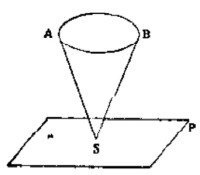
\includegraphics[scale=.5]{a20210131ThanksfortheMemories-img001.jpg} 
\caption{Memory Cone}
\end{wrapfigure}

The esoteric teaching is that forgetting is analogous to sleeping and to death, as they manifest on different levels. Valentin Tomberg makes it clear:

\begin{quotex}
For our whole experience (outer and inner) forgetting, sleep and death are three manifestations of the same thing —namely the “thing” which effects disappearance. It is said that sleep is the younger brother of death. It is necessary to add: forgetting is the brother of sleep. … One forgets, one goes to sleep, and one dies. One remembers, one awakes, and one is born. Remembering is to forgetting as awakening is to falling asleep, and awakening is to sleeping as birth is to death. … Natural forgetting reduces man to animality; natural sleep reduces him to vegetality; and natural death reduces him to minerality. 

\flright{\textit{Letter XIII, Death}}

\end{quotex}

Yet remembering is not simply bringing an image of the past into the present, since there are levels of depth to memory. You can remember solely with the intellect, with feelings, or even with the will. The highest is moral memory, based on love and all that accompanies it. Tomberg emphasizes the importance of the latter:

\begin{quotex}
It is love which is at work in moral memory when it recalls things from the past. Here it is admiration, respect, friendship, gratitude, affection and a thousand other things which have deeply moved you, which render things from the past unforgettable, i.e., evocable at each instant. The more one has loved, the more one remembers through moral memory.

Moral memory — which can comprehend everything without exception — is all the more effective the less one is morally indifferent. Indifference, a lack of moral interest, is the fundamental cause of the lapse of memory which often takes place in old age. The less one is indifferent, the more one remembers of the past and the more one is capable of learning new things. 

\end{quotex}
\paragraph{Moral Memory}
Moral memory predominates in old age. The young depend on mechanical memories, which arise spontaneously; this faculty becomes feebler with age. Hence, it must be replaced with intellectual or logical memory. This requires an active effort to remember things. People who neglected to learn how to make intellectual efforts in their youth, will become forgetful as they age. Tomberg goes even further, explaining that moral efforts are likewise necessary:

\begin{quotex}
People who are able to and who know how to give everything a moral worth and to see a moral sense in everything will not forget anything: they will have a normal, if not excellent, memory to a very advanced age.

Moral memory — which can comprehend everything without exception — is all the more effective the less one is morally indifferent. Indifference, a lack of moral interest, is the fundamental cause of the lapse of memory which often takes place in old age. The less one is indifferent, the more one remembers of the past and the more one is capable of learning new things. 

\end{quotex}
\paragraph{Love and Work}
\begin{quotex}
Love and work are the cornerstones of our humanness. \flright{\textsc{Sigmund Freud}}

\end{quotex}
To begin the experiment of “remembering”, one must first decide what to remember. If love and work are the cornerstones of our humanness, that is the place to start. When one loves, one cannot be morally indifferent. And our acts — our work, our projects, our adventures — only have significance when they are moral acts. So we turn to our favorite Knight Errant, Don Quixote, who had expertise in both realms, as a model.

Love was constantly on his mind, especially for the one special lady, who was the driving force, the creative force, for his life. He treated women with chivalry. Against men, he was prepared to do battle against iniquity and to protect the weak and helpless. He brandished his cold weapons to make a point. He did not carry around a copy of the constitution nor did he propose to reason with his enemies to make his point. That is why his deeds have been recorded and are remembered.

\paragraph{Pointillism}
Most people live their lives as an accumulation of points, one after the other. Events in their lives are unrelated to each other since points are unrelated. They are stuck in time and not in simultaneity. If you desire to live your life as a work of art, whom would you commission to paint it for you?

The realist will plan it in advance: he will make a detailed drawing, calculate the perspectives, choose the colours, lighting, etc. The end result is known even before the artist begins. The unsophisticated viewer prefers realism because it requires little or no effort from him.

The better choice is pointillism. As you live your life day to day, it is difficult to grasp it as a whole. Instead, your life appears to you as a series of points of various colours, almost at random, and it may not make sense as a whole at any given time. However, as the points are painted at various spots on the canvas, gradually the full image of your life can be discerned. But this takes more effort — and patience — by the viewer to wait for the points to begin to make sense.

So that is how to start, each memory is a point or set of related points. Over time, as they appear on the canvas of your life, the whole picture of your life should come into view.

\paragraph{Life is Short}
They say that life is too short. Your memories should be relevant; they should be predominantly moral memories. If your fondest memories are watching TV or hanging out at the pub, then your life is actually too long and you are trying to fill it up with trivialities.

To develop a moral memory, you must live by principles and your acts must have a point. This should be obvious, for the alternative is live a life that is unprincipled and pointless.

\paragraph{Dislikes, Fears, and Accidents}
The first step in deep remembering is to ascertain one's earliest likes, talents, and proclivities. This exercise is preferable to most people because it seems pleasant. However, one can gain more self-knowledge by remembering the things you did not like. What events transpired in your life that you did not desire? Can you see what role, however subtle, you may have played in bringing it about?

This applies also to what you most fear. How has the avoidance of this fear shaped your life?

Another consideration is to remember everything that occurred, seemingly by chance or accident. From the human point of view, that may seem to be the case. But can you dig even deeper to see if there is a state of being from which you willed those events.

Meditations like these will often bear great fruit.

\paragraph{Encounters with Others}
Your life is a world line in the cosmos. And everyone else has his own world line. Mathematically understood, a Point is where two Lines intersect. In other words, the points don't define the line, but the line defines the points that constitute it.

So when I see a Point, I don't ask what it means in isolation. Instead, I look for the two lines. Of course, you are one of them, and the other is a person you encounter. Why are two distinctly different world lines meeting at that point? From that perspective, you can experience the event in its wholeness, all at once, simultaneously.

There are natural reasons, of course, for the intersection of lines: family, jobs, food, love, revenge, and so on, i.e., all the things involved in human life. But that does not exhaust all the possibilities.

Nevertheless, some lines meet for no human purpose at all, yet you can't dismiss it as pointless because the Point is there and is unavoidable. You may choose to look away. That is possible because it is so ethereal. But that decision has its danger, since you may miss one of the most important moments in your life.

How many of those life events have you forgotten? and you may even be glad they are forgotten. How few of those memories will endure through eternity? It is imperative to know what to forget and what to remember.

Why have some people made an impact on your life and others not so much?

\paragraph{Things forgotten}
You will find memories best left forgotten. Something that had seemed so important and so impactful at that time, appears now in retrospect to be so distant, so far from your current level of being, that it may as well have been the memory of a different person. It may remain as an intellectual memory, but it no longer has any emotional impact, and it most certainly does not induce you to act.



\flrightit{Posted on 2021-01-31 by Cologero }

\begin{center}* * *\end{center}

\begin{footnotesize}\begin{sffamily}



\texttt{Michael M on 2021-01-31 at 10:26 said: }

“They say that life is too short. Your memories should be relevant; they should be predominantly moral memories. If your fondest memories are watching TV or hanging out at the pub, then your life is actually too long and you are trying to fill it up with trivialities.

To develop a moral memory, you must live by principles and your acts must have a point. This should be obvious, for the alternative is live a life that is unprincipled and pointless.”

You describe exactly my experience lately when I hear someone say “killing time”. Internally I watch my cage intensely when I see it in others and am watchful for it in my own domain. Quite insidious a phrase especially when understanding time as part of the compound nature of experience, life, and the unfolding of ideas. Don't want to fall asleep in a dream and dream our life away…

Has anyone found it more difficult at times to remember “facts” (academic / intellectual) memories when focusing on moral memory intensely? Or perhaps there is some type of learning curve or displacement of useless knowledge for rewriting of moral orientation?


\end{sffamily}\end{footnotesize}
